% ═══════════════════════════════════════════════════════════════════════════
% Chapter 6: Host Software Architecture
% ═══════════════════════════════════════════════════════════════════════════

\chapter{Host Software Architecture} \label{chap:host}

\section{Overview}

The host-side software is a C++17 application built with CMake, providing real-time data ingestion, sensor fusion, rep segmentation, visualization, and persistent storage. The codebase is organized into modular components following the Signal-Slot pattern for decoupled communication.

\section{Directory Structure}

\begin{verbatim}
src/
├── app/
│   ├── Application.h/cpp    # Application lifecycle
│   └── Config.h/cpp         # Configuration management
├── core/
│   ├── Session.cpp/cpp      # Session state management
│   └── SyncEngine.cpp/cpp   # IMU-Camera synchronization
├── gui/
│   ├── MainWindow.cpp/cpp   # Main application window
│   ├── SensorPanel.cpp/cpp  # Real-time sensor visualization
│   ├── PlotPanel.cpp/cpp    # Time-series plotting
│   └── AnnotationPanel.cpp/cpp  # Rep annotation interface
├── processing/
│   └── RepSegmenter.cpp/cpp # Rep boundary detection
├── annotation/
│   ├── SessionLibrary.cpp/cpp  # Session browser
│   └── VideoCache.cpp/cpp     # Video preloading
└── sensors/
    ├── IMUReader.cpp/cpp    # ESP-NOW data ingestion
    └── CameraReader.cpp/cpp # RealSense integration
\end{verbatim}

\section{Application Lifecycle}

\subsection{Initialization Sequence}

\begin{lstlisting}[language=c++]
bool Application::init(int argc, char** argv) {
    // 1. Parse command-line arguments
    if (!parseArgs(argc, argv)) return false;

    // 2. Load configuration from disk
    Config::load("vbt_config.json");

    // 3. Initialize logging (spdlog)
    initLogging();

    // 4. Set up signal handlers for graceful shutdown
    setupSignalHandlers();

    // 5. Initialize sensor subsystems
    if (!imuReader_->init()) {
        spdlog::error("IMU reader initialization failed");
        return false;
    }

    if (!cameraReader_->init()) {
        spdlog::error("Camera reader initialization failed");
        return false;
    }

    // 6. Initialize GUI (if not headless)
    if (!config_.headless) {
        gui::MainWindow mainWindow;
        mainWindow.show();
    }

    return true;
}
\end{lstlisting}

\section{Real-Time Data Ingestion}

\subsection{ESP-NOW Receiver}

The IMU reader implements a UDP-like protocol over ESP-NOW for barbell telemetry:

\begin{lstlisting}[language=c++]
class IMUReader {
public:
    bool init() {
        espnow_init();
        esp_now_register_recv_cb([](uint8_t* mac, uint8_t* data, int len) {
            getInstance()->onDataReceived(mac, data, len);
        });
        return true;
    }

    void onDataReceived(uint8_t* mac, uint8_t* data, int len) {
        auto payload = reinterpret_cast<espnow_payload_t*>(data);

        IMUSampleBatch batch;
        batch.timestamp_us = esp_timer_get_time();
        batch.sequence = payload->sequence;

        for (int i = 0; i < SAMPLE_BATCH_SIZE; i++) {
            batch.samples[i] = {
                accel_x: payload->accel_x[i],
                accel_y: payload->accel_y[i],
                accel_z: payload->accel_z[i],
                gyro_x: payload->gyro_x[i],
                gyro_y: payload->gyro_y[i],
                gyro_z: payload->gyro_z[i],
            };
        }

        // Emit signal to processing pipeline
        onNewBatch_(batch);
    }

private:
    sig::signal<void(const IMUSampleBatch&)> onNewBatch_;
};
\end{lstlisting}

\subsection{Camera Integration}

The RealSense pipeline uses librealsense for depth and color streams:

\begin{lstlisting}[language=c++]
bool CameraReader::init() {
    pipe_ = std::make_unique<rs2::pipeline>();
    rs2::config cfg;
    cfg.enable_stream(RS2_STREAM_DEPTH, 640, 480, RS2_FORMAT_Z16, 90);
    cfg.enable_stream(RS2_STREAM_COLOR, 640, 480, RS2_FORMAT_BGRA8, 90);

    rs2::config::enable_stream(RS2_STREAM_FSYNC, RS2_FSYNC_MODE_TOGGLING);

    profile_ = pipe_->start(cfg);
    return true;
}

std::optional<CameraFrame> CameraReader::grabFrame(int timeout_ms) {
    rs2::frameset frames = pipe_->wait_for_frames(timeout_ms);

    auto depth = frames.get_depth_frame();
    auto color = frames.get_color_frame();
    auto fsync = frames.get_frame(RS2_STREAM_FSYNC);

    CameraFrame frame;
    frame.depth_data = static_cast<uint16_t*>(depth.get_data());
    frame.color_data = static_cast<uint8_t*>(color.get_data());
    frame.fsync_timestamp_us = fsync.get_timestamp();
    frame.sequence = fsync.get_frame_number();

    return frame;
}
\end{lstlisting}

\section{Session Management}

\subsection{Session State Machine}

\begin{figure}[h]
    \centering
    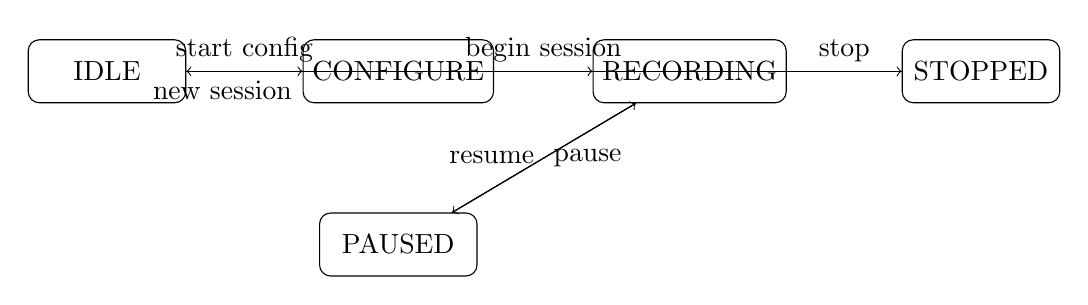
\begin{tikzpicture}[node distance=1.2cm, auto]
        \tikzstyle{state}=[draw, rectangle, rounded corners, minimum width=2cm, minimum height=0.8cm];

        \node[state] (idle) {IDLE};
        \node[state, right of=idle, xshift=2.5cm] (config) {CONFIGURE};
        \node[state, right of=config, xshift=2.5cm] (recording) {RECORDING};
        \node[state, below of=config, yshift=-1cm] (paused) {PAUSED};
        \node[state, right of=recording, xshift=2.5cm] (stopped) {STOPPED};

        \draw[->] (idle) -- node[midway, above] {start config} (config);
        \draw[->] (config) -- node[midway, above] {begin session} (recording);
        \draw[->] (recording) -- node[midway, right] {pause} (paused);
        \draw[->] (paused) -- node[midway, left] {resume} (recording);
        \draw[->] (recording) -- node[midway, above] {stop} (stopped);
        \draw[->] (stopped) -- ++(-5.5,0) |- node[pos=0.95, below] {new session} (idle);
    \end{tikzpicture}
    \caption{Session state machine}
    \label{fig:session_state}
\end{figure}

\subsection{Session Metadata}

Each session persists a schema-versioned JSON manifest:

\begin{lstlisting}[caption={Session metadata JSON schema}]
{
  "schema_version": "4.0.0",
  "session_id": "session_20260510_121411",
  "start_time_utc": "2026-05-10T12:14:11.234Z",
  "exercise": "snatch",
  "athlete": {
    "subject_id": "SUBJ_001",
    "sex": "M",
    "age_years": 28,
    "height_cm": 178,
    "weight_kg": 82,
    "training_age_years": 5
  },
  "training_context": {
    "session_date": "2026-05-10",
    "phase": "mesocycle_3_accumulation",
    "set_number": 3,
    "target_reps": 5,
    "load_kg": 70,
    "rpe": 7,
    "rest_between_sets_s": 180
  },
  "equipment": {
    "barbell": "rogue_olympic_20kg",
    "collars": "elum_collars",
    "im_u_serial": "ICM42688P_28A3F1",
    "camera_serial": "876412072345"
  },
  "data_files": {
    "imu_csv": "imu/raw_imu.csv",
    "video_mp4": "video/color.mp4",
    "depth_npy": "depth/depth.npy",
    "annotations_json": "annotations/rep_segments.json"
  }
}
\end{lstlisting}

\section{Real-Time Visualization}

\subsection{Sensor Panel}

The SensorPanel displays live IMU telemetry with configurable scalar/vector plots:

\begin{figure}[h]
    \centering
    \framebox[\width][c]{
        \begin{minipage}{0.8\textwidth}
            \centering
            [SensorPanel GUI Screenshot]\\
            - Accelerometer: X/Y/Z traces (0-10 s window)\\
            - Gyroscope: X/Y/Z traces\\
            - computed orientation Euler angles\\
            - Real-time velocity estimate\\
        \end{minipage}
    }
    \caption{SensorPanel real-time visualization}
    \label{fig:sensor_panel}
\end{figure}

\subsection{Plot Panel}

PlotPanel uses OpenGL-accelerated line rendering for high-sample-rate time series:

\begin{lstlisting}[language=c++]
void PlotPanel::render(const std::vector<Sample>& data) {
    glBindBuffer(GL_ARRAY_BUFFER, vbo_);
    glBufferData(GL_ARRAY_BUFFER,
                 data.size() * sizeof(GLfloat),
                 nullptr,
                 GL_DYNAMIC_DRAW);
    auto* ptr = (GLfloat*)glMapBuffer(GL_ARRAY_BUFFER, GL_WRITE_ONLY);

    for (size_t i = 0; i < data.size(); i++) {
        ptr[2*i] = static_cast<GLfloat>(data[i].time_s - t_start);
        ptr[2*i + 1] = static_cast<GLfloat>(data[i].value);
    }

    glUnmapBuffer(GL_ARRAY_BUFFER);

    glDrawArrays(GL_LINE_STRIP, 0, data.size());
}
\end{lstlisting}

\section{Data Persistence}

\subsection{CSV Export Format}

Raw IMU data persists in schema-versioned CSV:

\begin{verbatim}
unified_time_s,esp_timestamp_us,host_timestamp_s,
accel_x_g,accel_y_g,accel_z_g,gyro_x_dps,gyro_y_dps,gyro_z_dps
1715342051.234567,1205234567,1715342051.234890,
0.012,0.008,1.002,0.5,-0.2,0.1
\end{verbatim}

The \texttt{unified\_time\_s} column aligns IMU and camera timestamps using the FSYNC-based offset measured during the sync verification phase.

\section{Error Handling}

\subsection{Graceful Degradation}

The application handles sensor failures without data loss:

\begin{lstlisting}[language=c++]
void Session::onIMULoss() {
    spdlog::warn("IMU data stream interrupted");
    state_ = SessionState::IMU_DISCONNECTED;

    // Continue recording if camera available
    if (camera_->isConnected()) {
        spdlog::info("Continuing in camera-only mode");
        state_ = SessionState::RECORDING;
    }
}
\end{lstlisting}

\section{Logging and Diagnostics}

\subsection{Structured Logging}

The application uses spdlog with structured JSON output for machine-parseable diagnostics:

\begin{verbatim}
{"ts": "2026-05-10T12:14:11.234Z", "level": "INFO",
 "msg": "Session started", "session_id": "session_XXXX"}
{"ts": "2026-05-10T12:14:15.567Z", "level": "DEBUG",
 "msg": "IMU batch received", "seq": 4234, "latency_us": 88}
\end{verbatim}

\section{Summary}

This chapter presented the host software architecture including C++17 component design, real-time data ingestion from ESP-NOW and RealSense, session state management, visualization, and persistent storage. The modular design enables extensibility while maintaining real-time performance for 1 kHz IMU and 90 fps camera data streams.

\newpage